\documentclass{article}

\usepackage{graphicx}

\usepackage{caption}
\usepackage{subcaption}

\begin{document}

\begin{figure}[]
  \captionsetup[subfigure]{position=b}
  \centering 
  \begin{subfigure}[p]{0.45\textwidth}
    \centering
    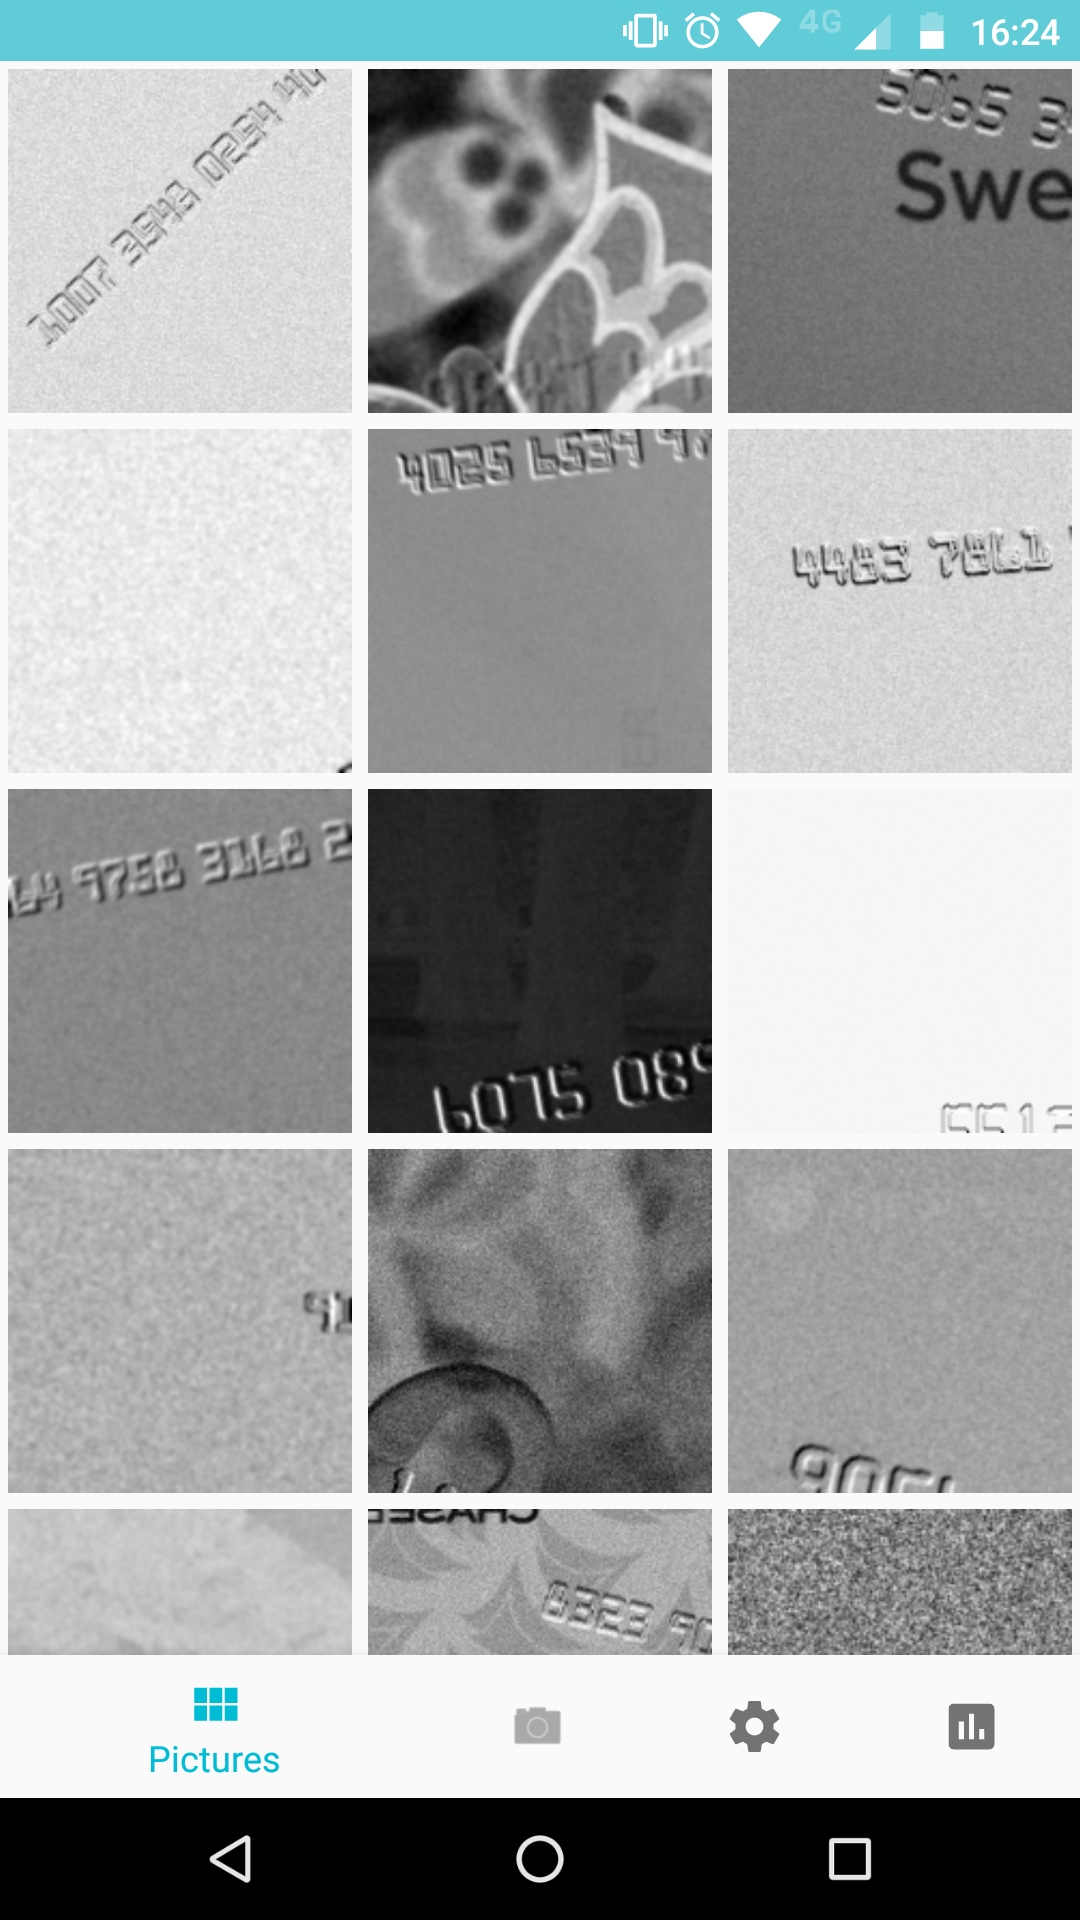
\includegraphics[width=0.75\textwidth]{img/app/main.png}
    \caption{\footnotesize MainActivity: presents a grid with pictures which will be run on the models when clicked.}
    \label{fig:MainActivity}
  \end{subfigure}
  \quad
  \begin{subfigure}[p]{0.45\textwidth}
    \centering
    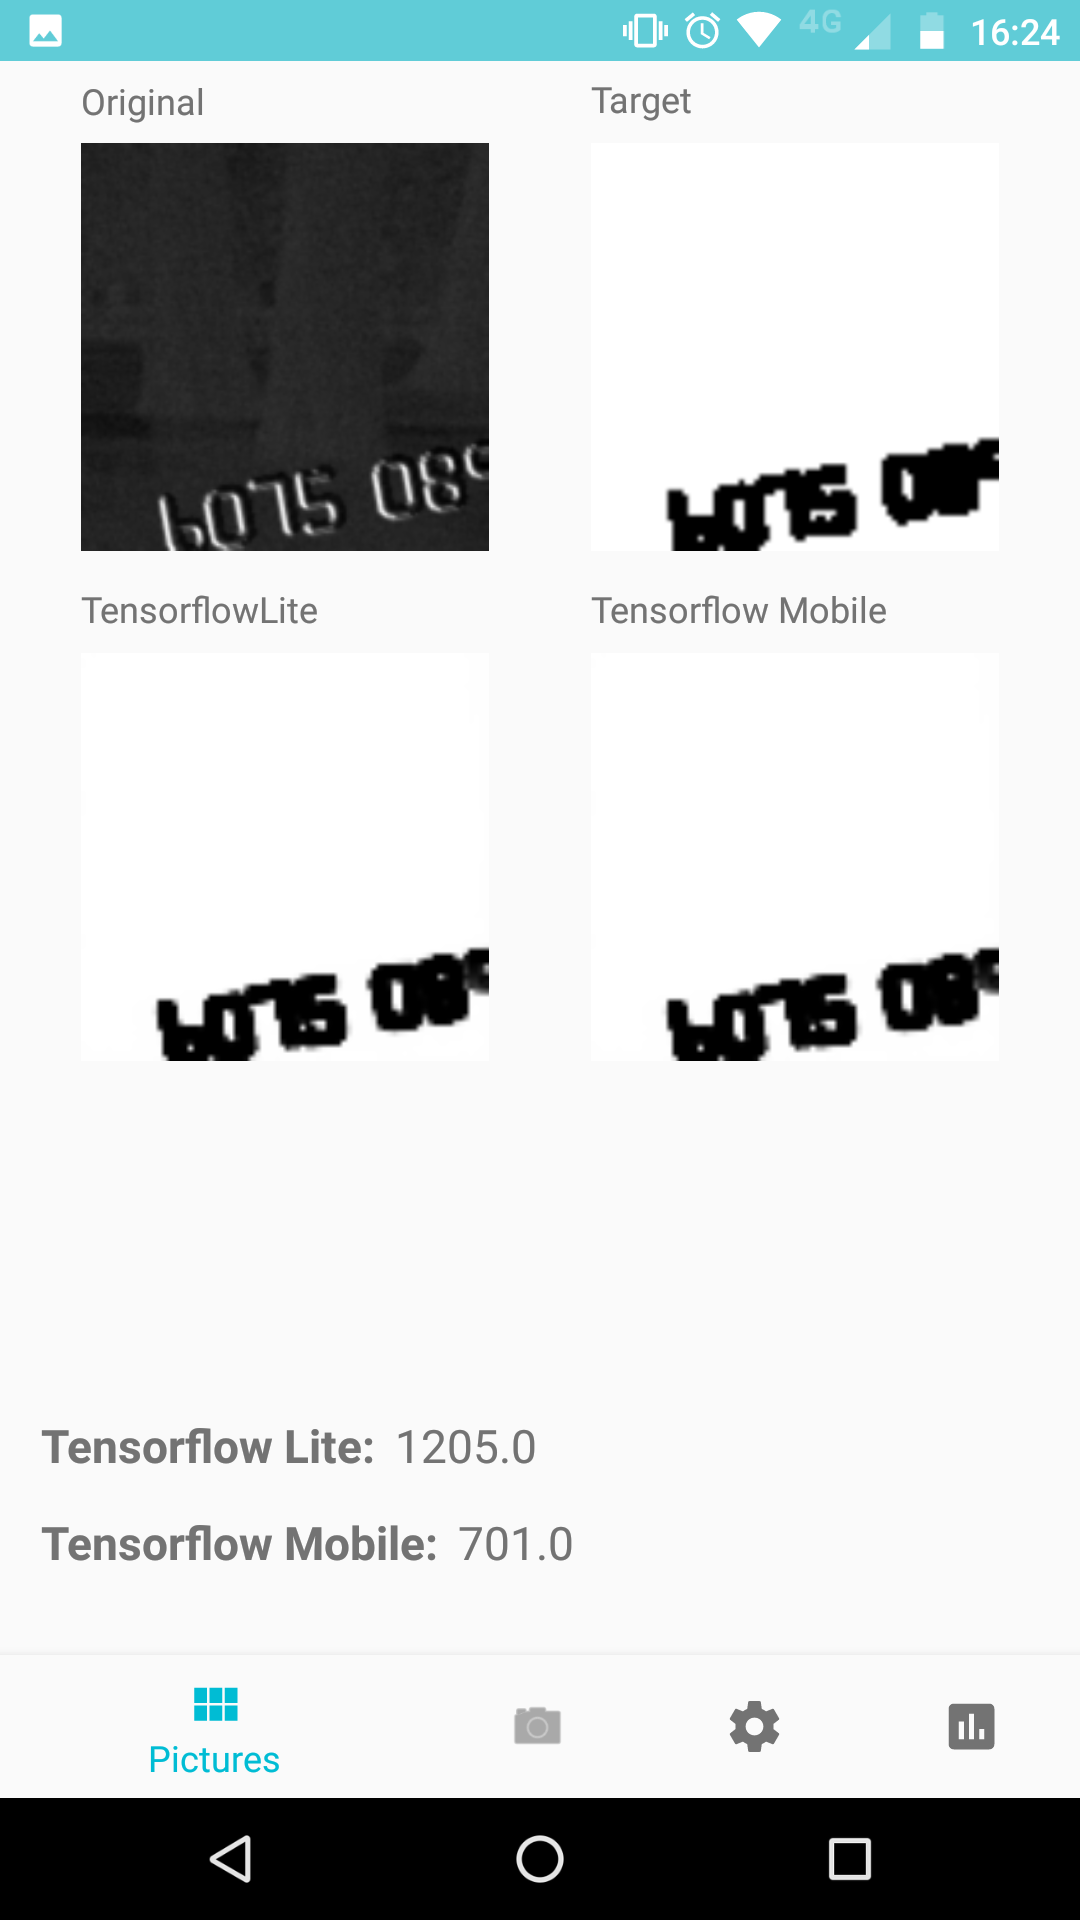
\includegraphics[width=0.75\textwidth]{img/app/display.png}
    \caption{\footnotesize DisplayActivity: after running the model displays the input picture, the target and the predictions of the models with their inference times.}
    \label{fig:DisplayActivity}
  \end{subfigure}
  \newline
  \vskip\baselineskip
  \begin{subfigure}[p]{0.45\textwidth}
    \centering
    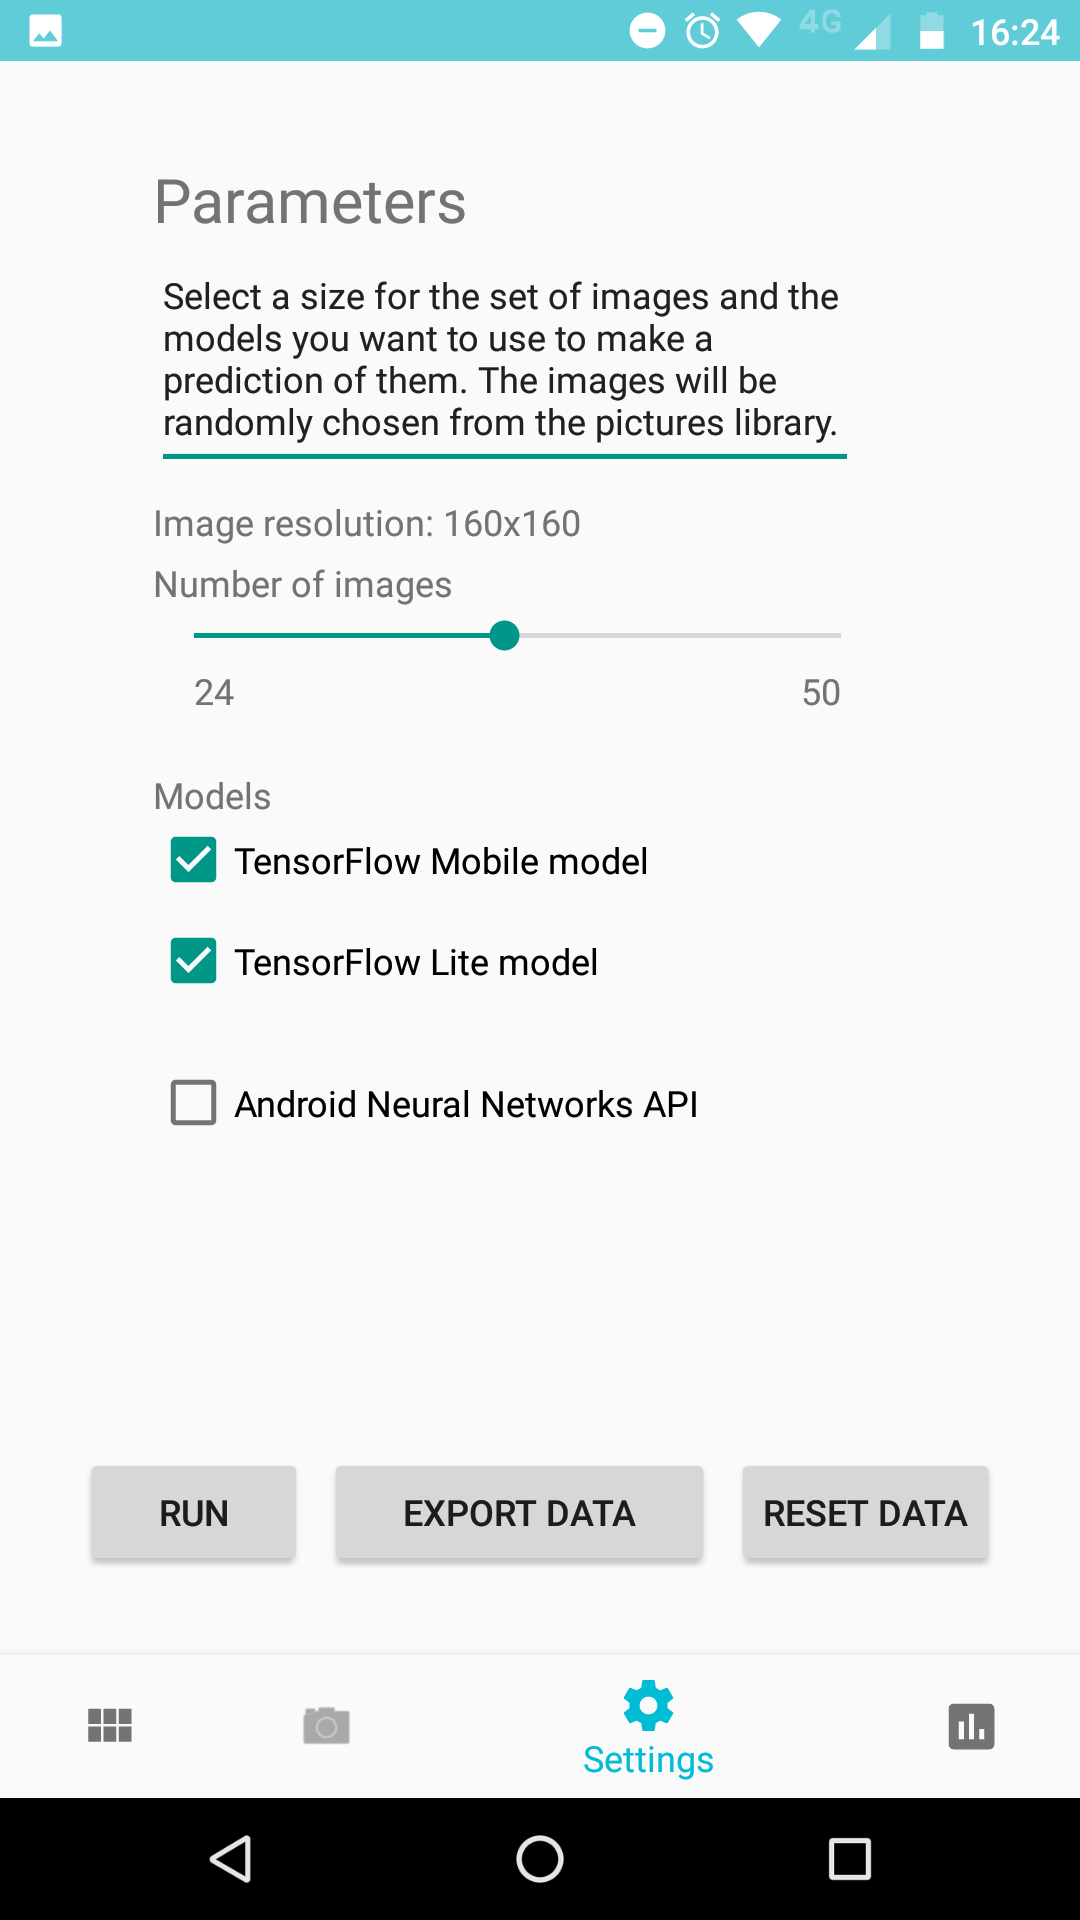
\includegraphics[width=0.75\textwidth]{img/app/settings.png}
    \caption{\footnotesize SettingsActivity: Menu to run the models on multiple images (number selected with the slider). The collected data points can be written to a file (export button) or erased (reset button).}
    \label{fig:SettingsActivity}
  \end{subfigure}
  \quad
  \begin{subfigure}[p]{0.45\textwidth}
    \centering
    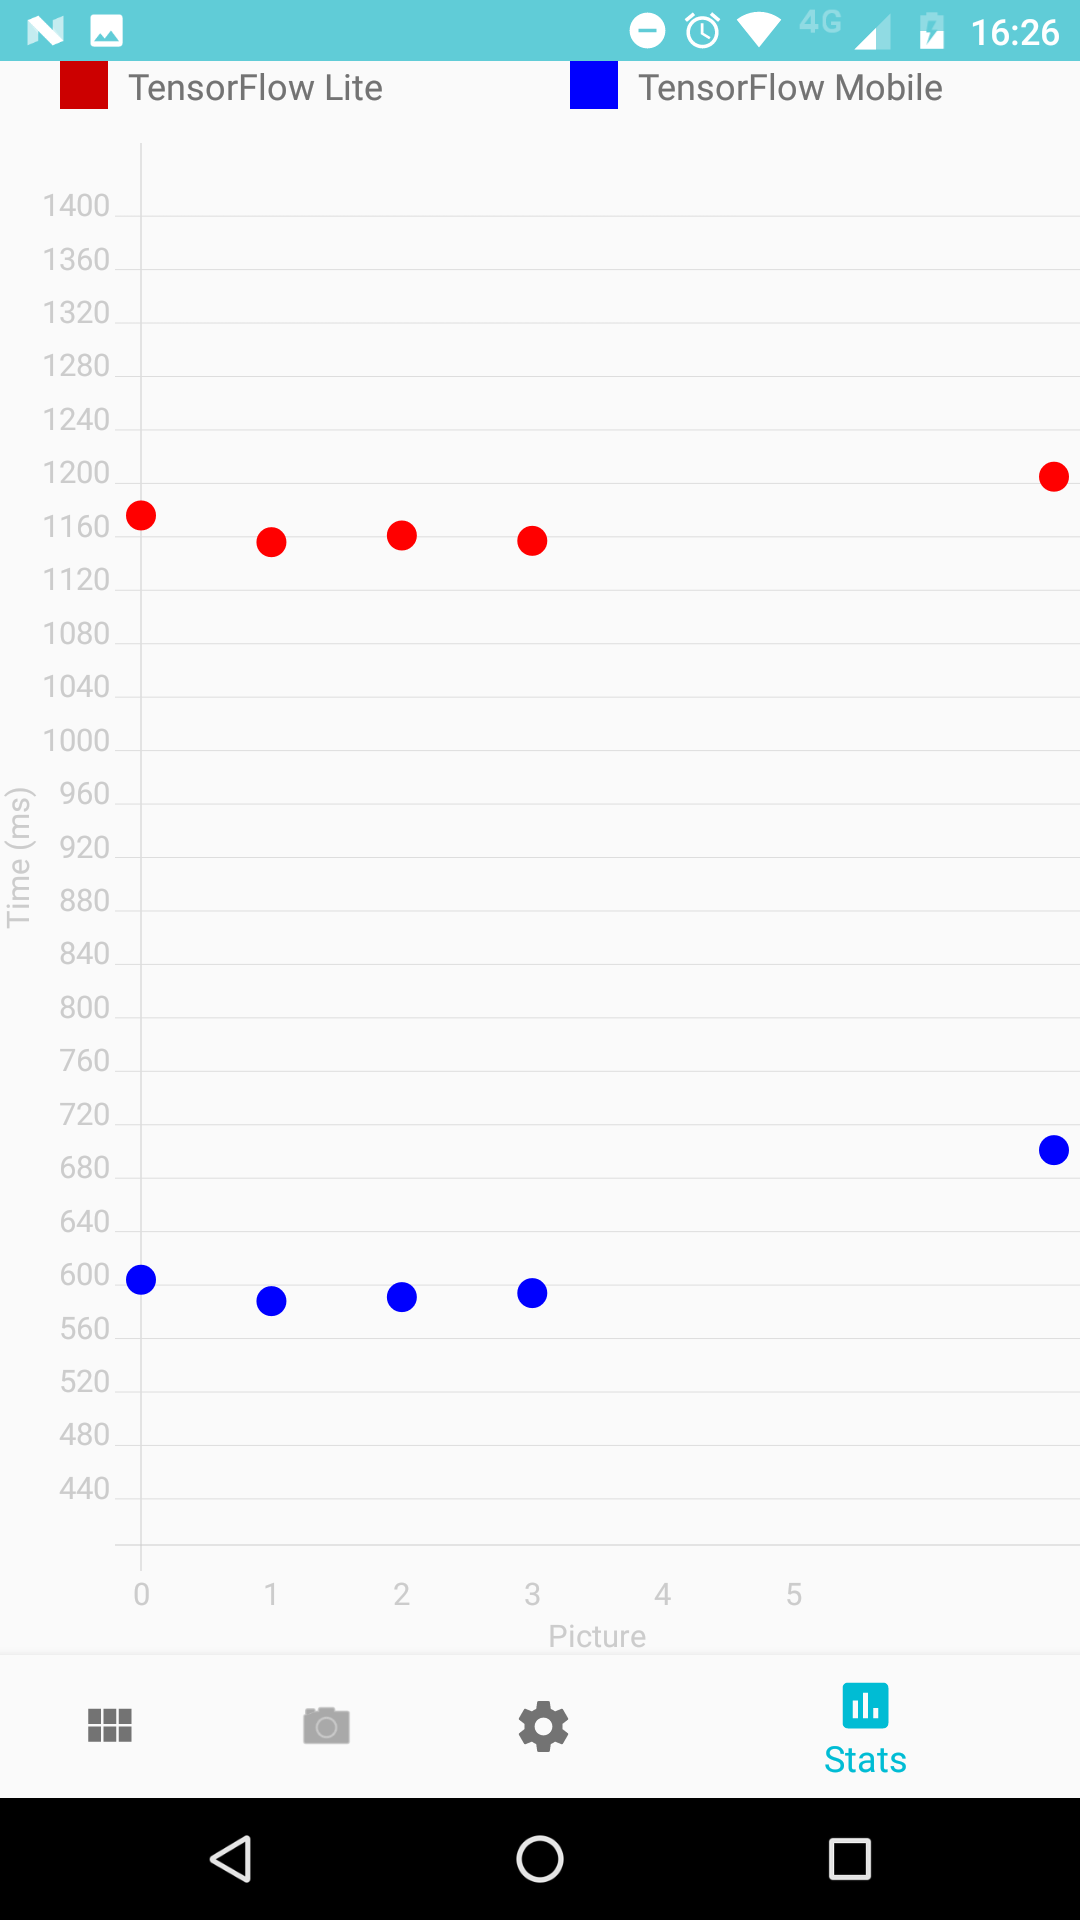
\includegraphics[width=0.75\textwidth]{img/app/stats.png}
    \caption{\footnotesize StatsActivity: displays a chart which compares the inference time between the two models for each image.}
    \label{fig:StatsActivity}
  \end{subfigure}
  \caption {\footnotesize Principal activities in test application}
  \label{fig:Activities}
\end{figure}

\newpage

\begin{figure}[!h]
\captionsetup[subfigure]{position=b}
  \centering
  \begin{tabular}[c]{cc}
    \begin{subfigure}[c]{0.4\textwidth}
      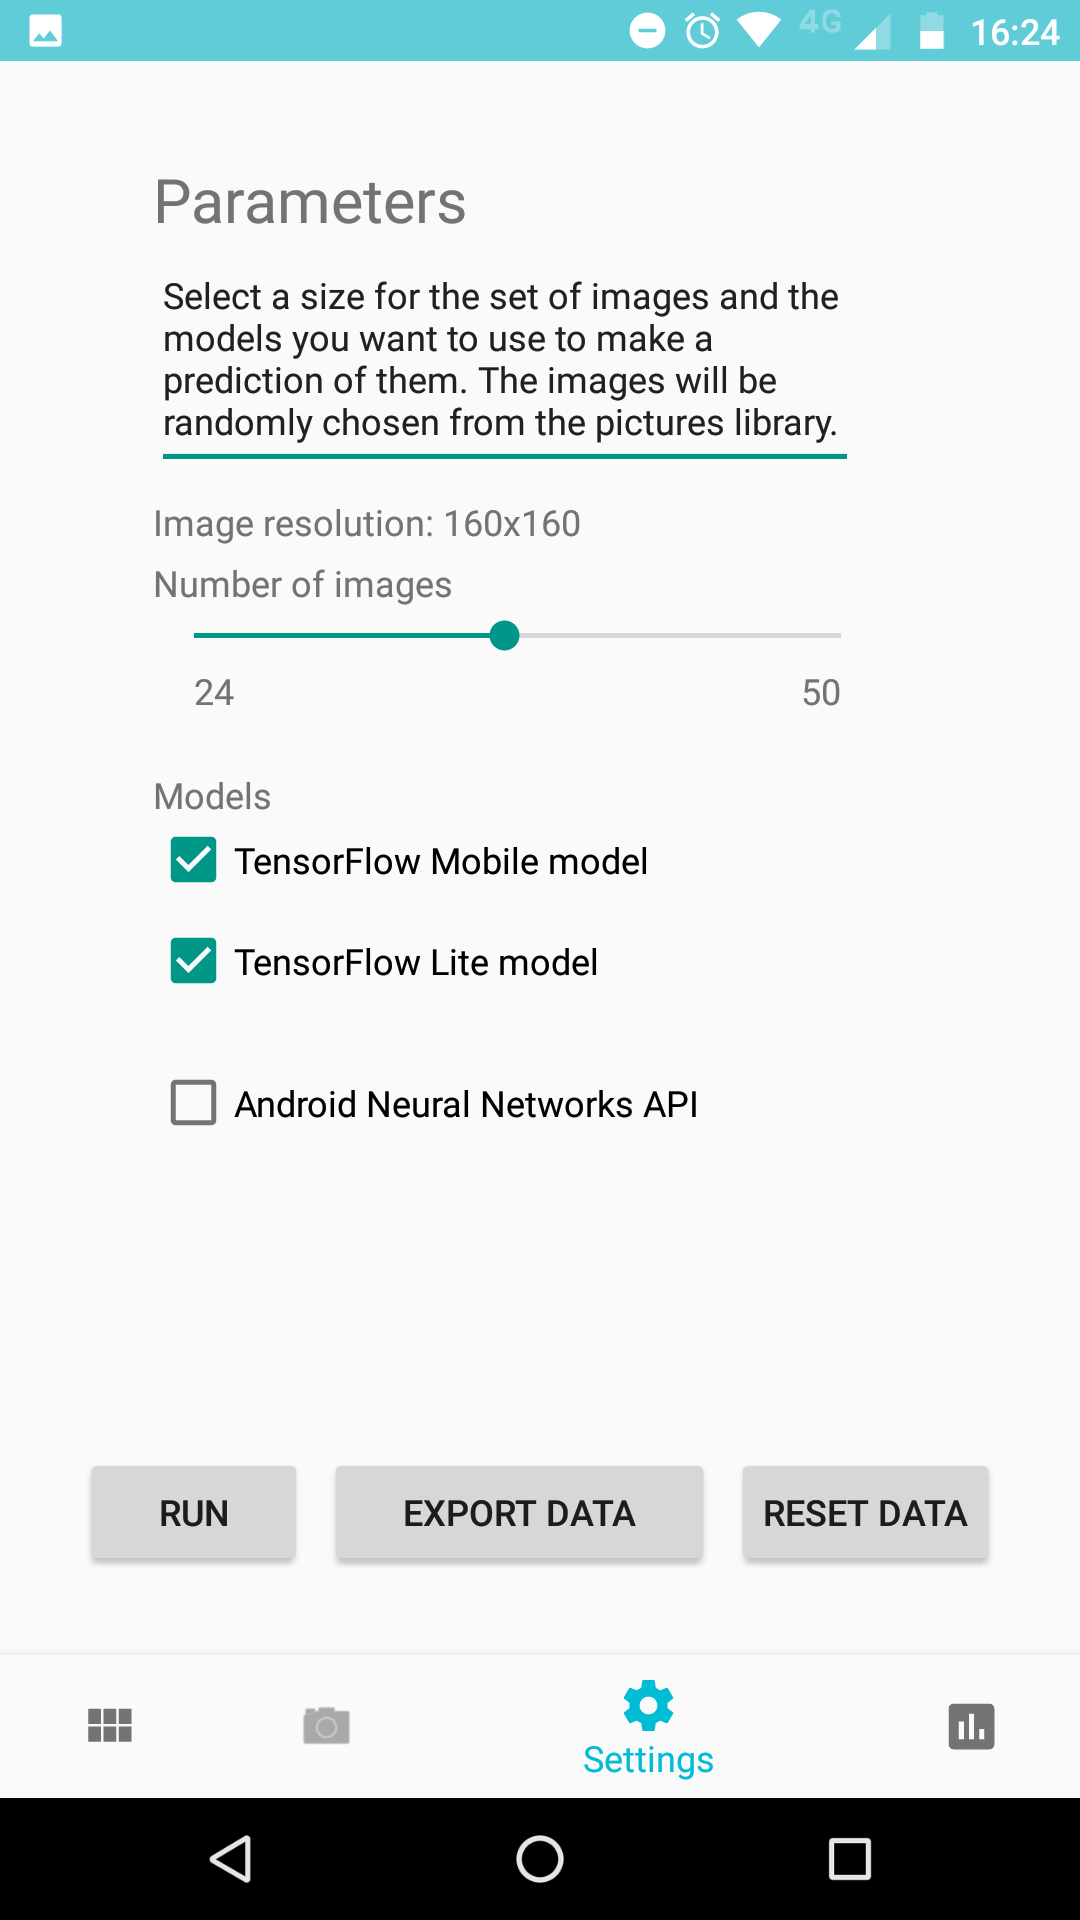
\includegraphics[width=\textwidth]{img/app/settings.png}
      \caption{figure}{\footnotesize MainActivity: presents a grid with pictures which will be run on the models when clicked.}
      \label{fig:MainActivity}
    \end{subfigure}&
    \begin{subfigure}[c]{0.4\textwidth}
      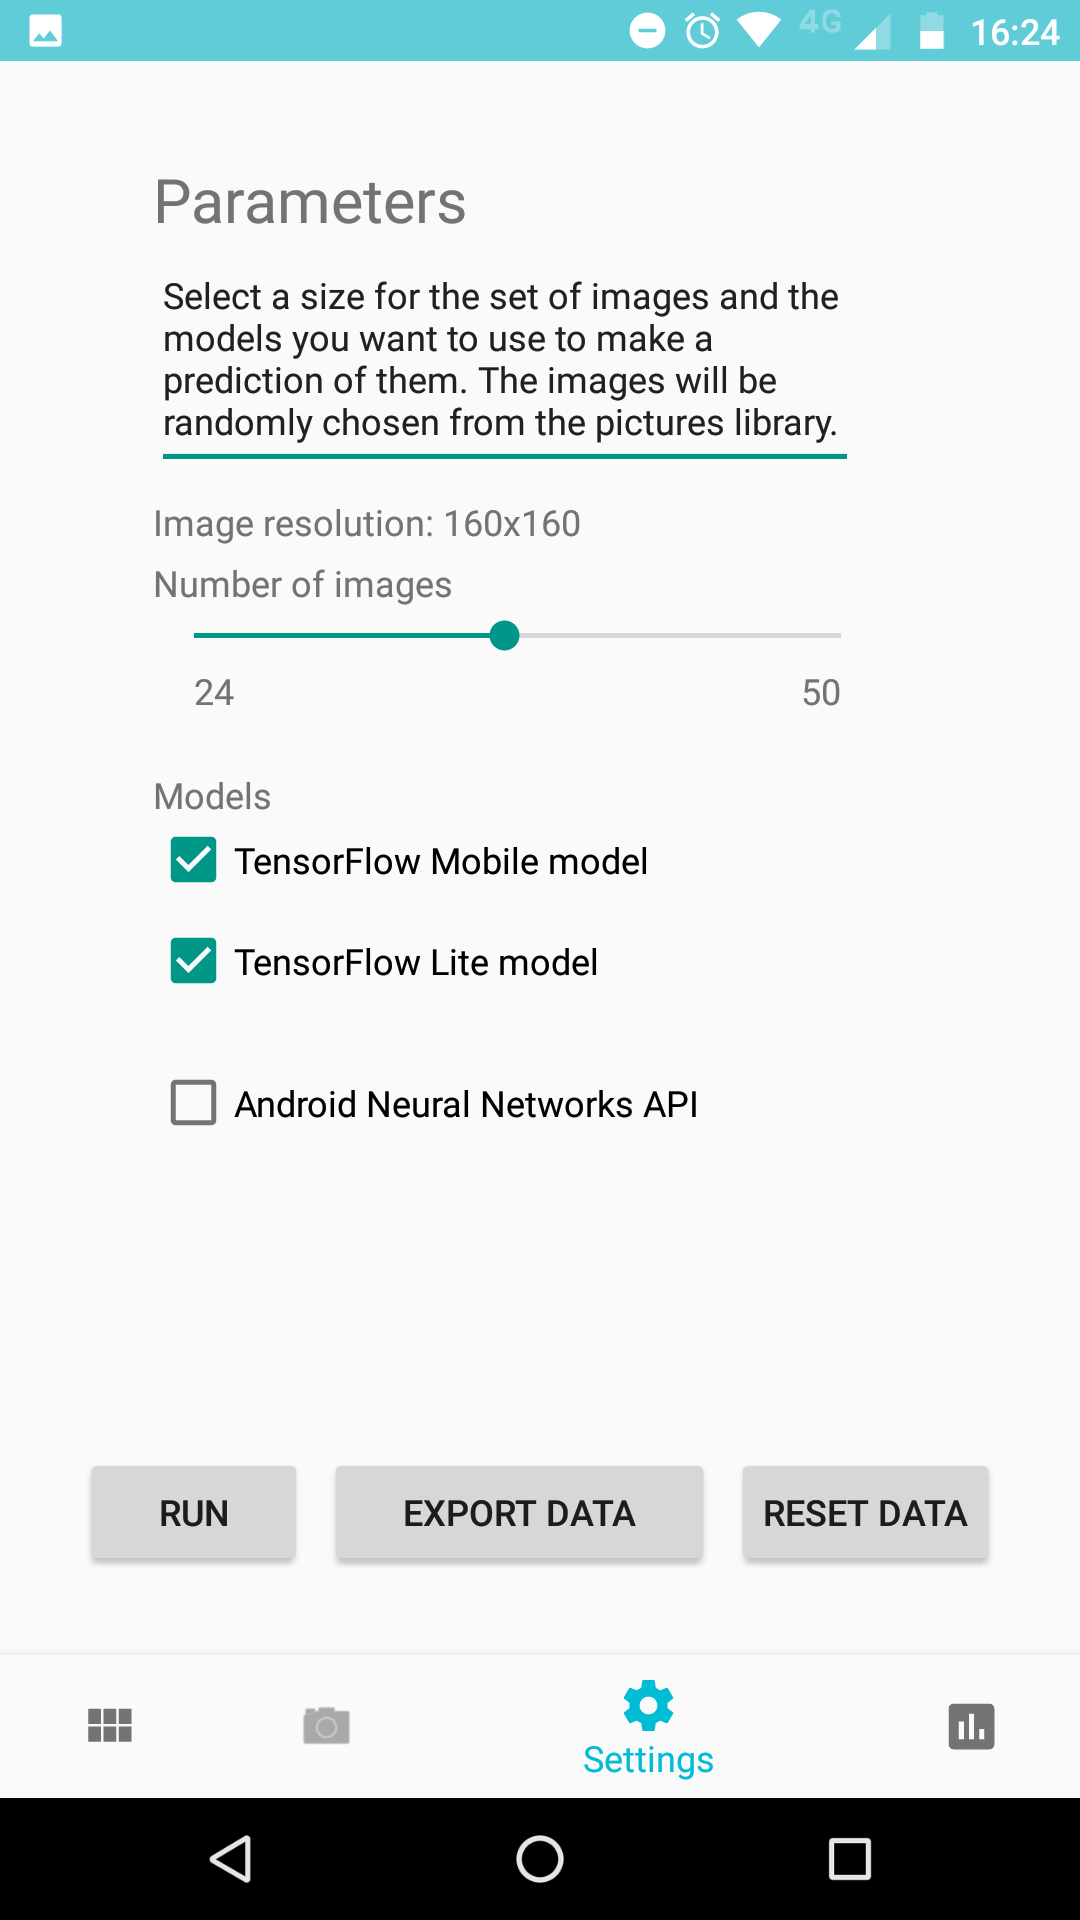
\includegraphics[width=\textwidth]{img/app/settings.png}
      \caption{figure}{\footnotesize DisplayActivity: after running the model displays the input picture, the target and the predictions of the models with their inference times.}
      \label{fig:DisplayActivity}
    \end{subfigure}\\

    \begin{subfigure}[c]{0.4\textwidth}
      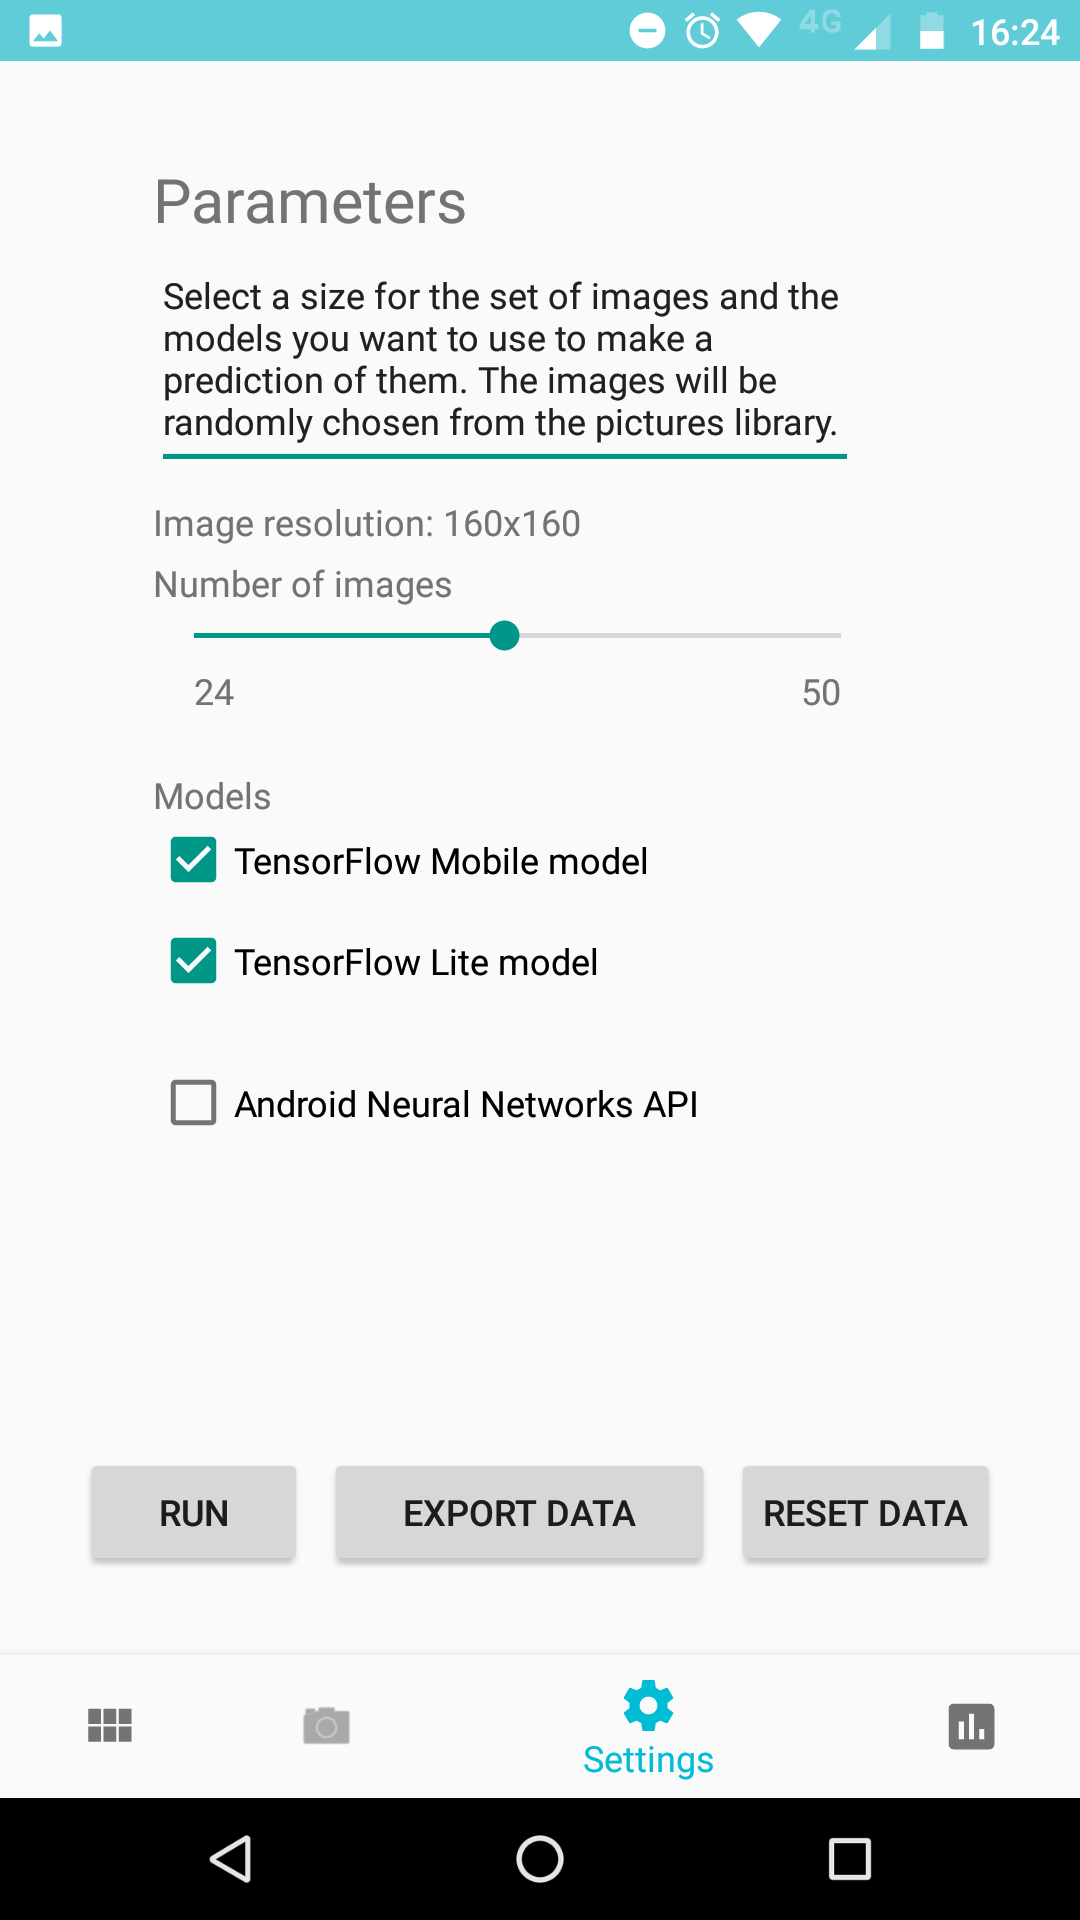
\includegraphics[width=\textwidth]{img/app/settings.png}
      \caption{figure}{\footnotesize SettingsActivity: Menu to run the models on multiple images (number selected with the slider). The collected data points can be written to a file (export button) or erased (reset button).}
      \label{fig:SettingsActivity}
    \end{subfigure}&
    \begin{subfigure}[c]{0.4\textwidth}
      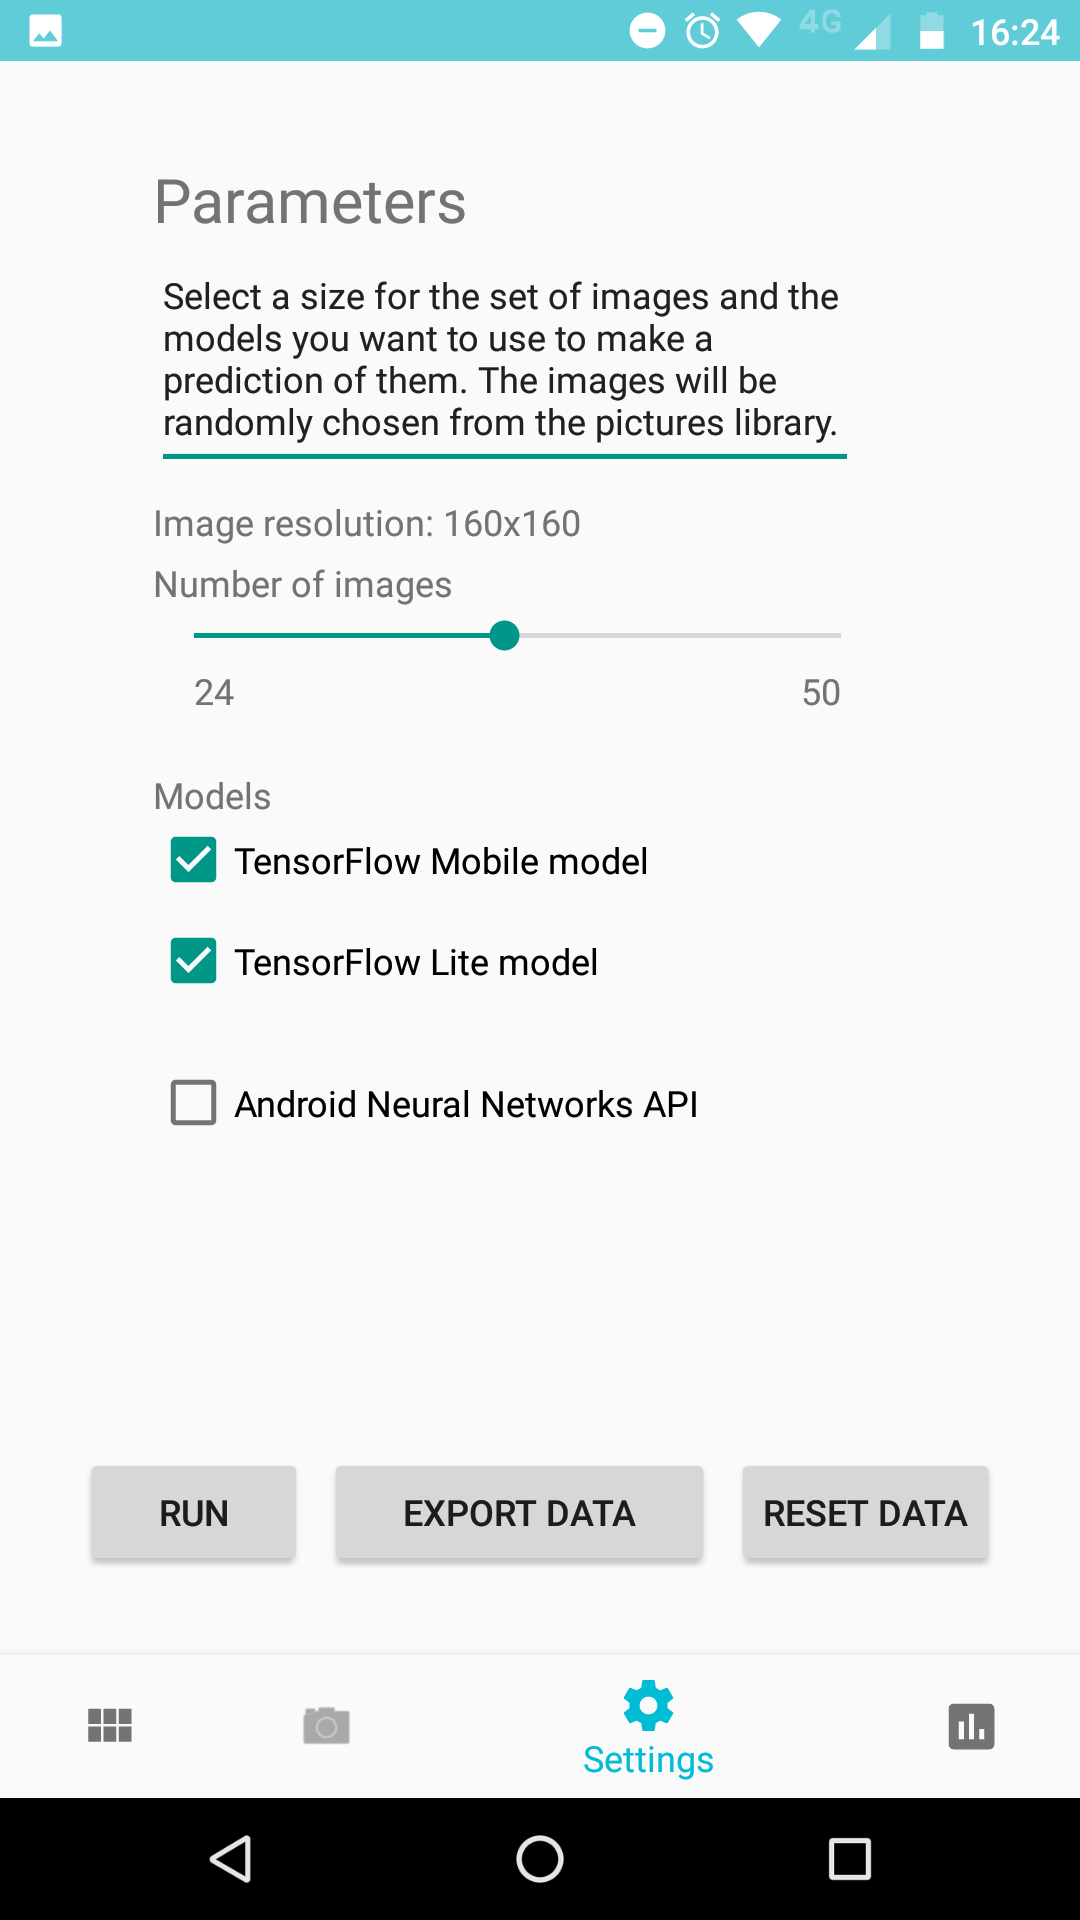
\includegraphics[width=\textwidth]{img/app/settings.png}
      \caption{figure}{\footnotesize StatsActivity: displays a chart which compares the inference time between the two models for each image.}
      \label{fig:StatsActivity}
    \end{subfigure}\\
  \end{tabular}    
  \caption{\footnotesize Principal activities in test application}
  \label{fig:Activities}
\end{figure}

\newpage 


\end{document}